\section{Introduction}

\begin{figure}[ht]
  \centering
  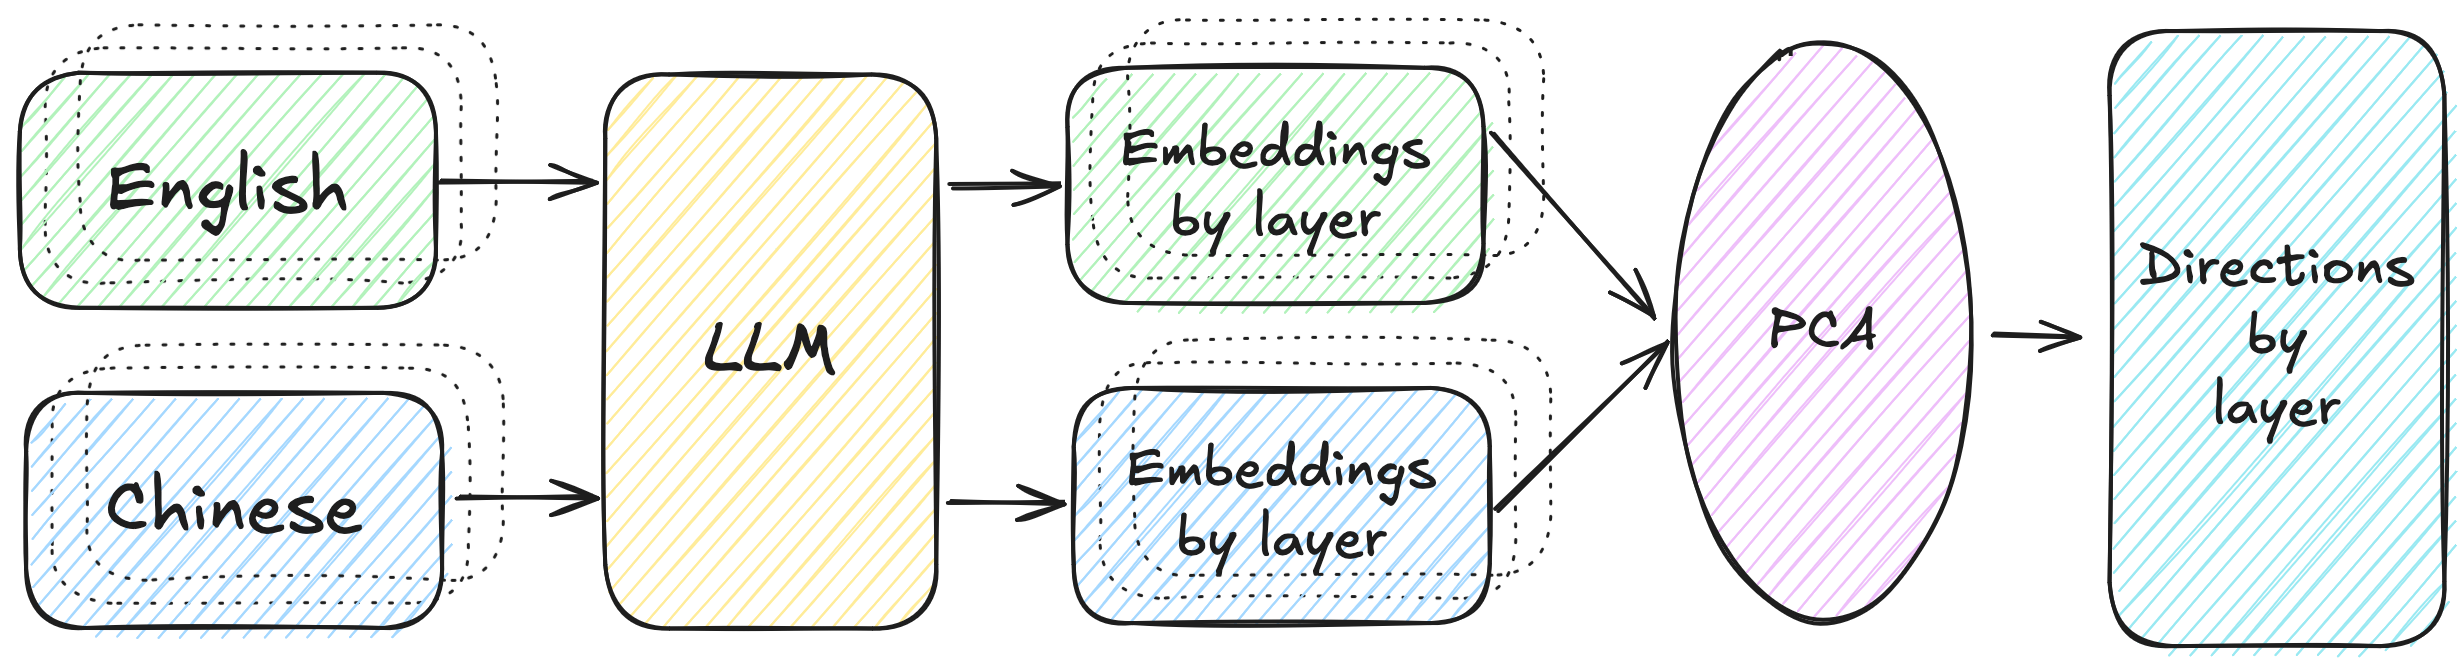
\includegraphics[width=1\linewidth]{images/language_steering_scheme.png}
  \caption{Language steering in hidden space: 1. Collect parallel translations of the same concepts; 2. LLM forward pass to get embeddings by layer; 3. Perform PCA by layer on the merged embeddings.}
  \label{fig:lang_steering_scheme}
\end{figure}

LLMs exhibit unintended code-switching - generating tokens in languages other than the target~\citep{marchisio-etal-2024-understanding}.
\citet{ryan-etal-2024-unintended} document how LLM alignment procedures can cause models to default to English even when prompted in other languages,
\citet{yoo2025codeswitchingredteamingllmevaluation} demonstrate that code-switching serves as an effective red-teaming vector, bypassing safety filters.
Existing solutions require costly fine-tuning~\citep{marchisio-etal-2024-understanding} or introduce latency via decoding-time interventions~\citep{dathathri2020plugplaylanguagemodels, yang-klein-2021-fudge, liu2021dexpertsdecodingtimecontrolledtext}.

We propose \emph{latent space language steering}, a cheap inference-time method that exploits low-dimensional language directions in hidden representations.
By applying PCA to parallel translations, we identify linear subspaces separating languages while preserving broad semantic direction.
Steering via simple projection (one dot product and vector subtraction per token) mitigates code-switching with negligible overhead.

Additionally, we analyze language clustering dynamics across layers and discover that a single final layer projection enables near-perfect language classification. Code and data are released to facilitate further research \footnote{\url{https://github.com/fxlrnrpt/language-steering-in-latent-space}}.
